\section{Rastreamento dos Usuários}

	O rastreamento é fundamental para o funcionamento correto do sistema uma vez que é responsável por rastrear os usuários no ambiente, determinar a sua localização física em relação ao sensor \textit{Kinect} e gerenciar suas identidades. Portanto, foi desenvolvido uma séries de testes funcionais para determinar suas limitações.

	Os primeiros testes realizados foram para testar a eficiência da detecção de novos usuários no ambiente. Os testes foram feitos simulando a entrada de um usuário na cena por diferentes ângulos e analisando o momento em que o mesmo era detectado. Em todos os testes o usuário era detectado antes mesmo de entrar na área de visão do sistema por completo, como mostrado na Figura~\ref{fig:testes_deteccao}.
	
		\begin{figure}[htb]
			\begin{center}
				\subfloat[] {
					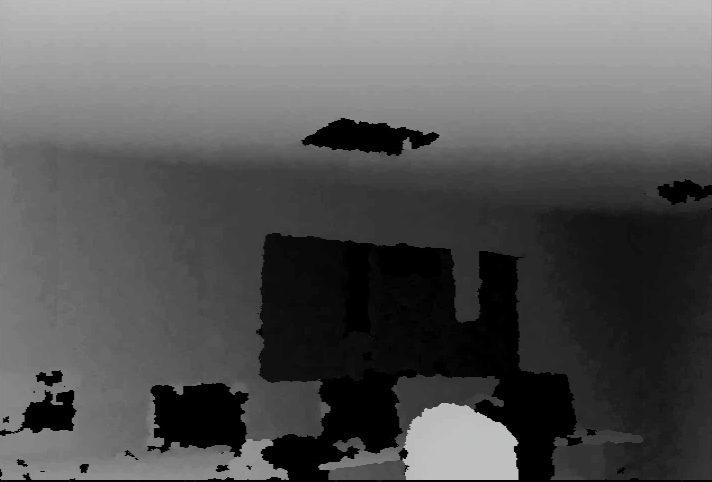
\includegraphics[width=0.25\textwidth]{figuras/5.Testes/deteccao/1.png}}
				\subfloat[] {
					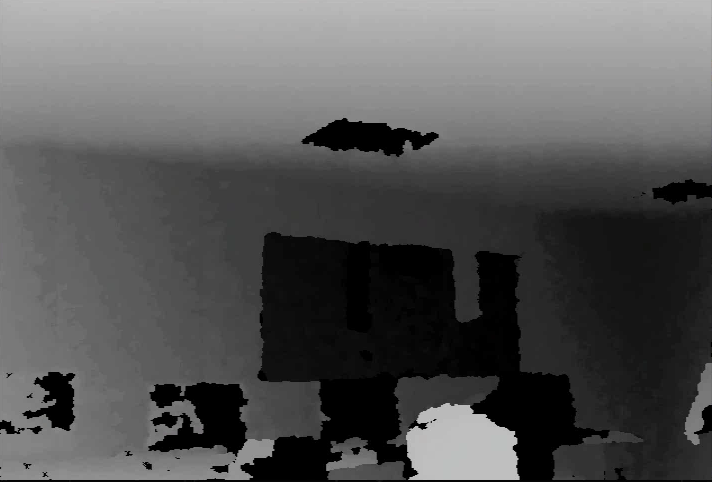
\includegraphics[width=0.25\textwidth]{figuras/5.Testes/deteccao/2.png}}
				\subfloat[] {
					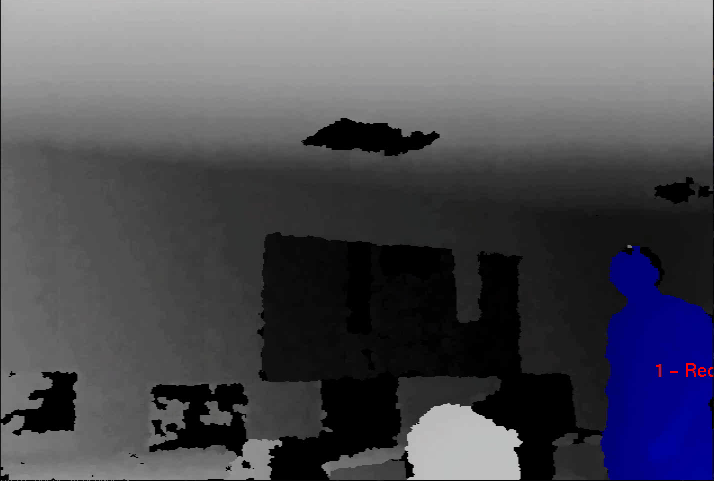
\includegraphics[width=0.25\textwidth]{figuras/5.Testes/deteccao/3.png}}
				\subfloat[] {
					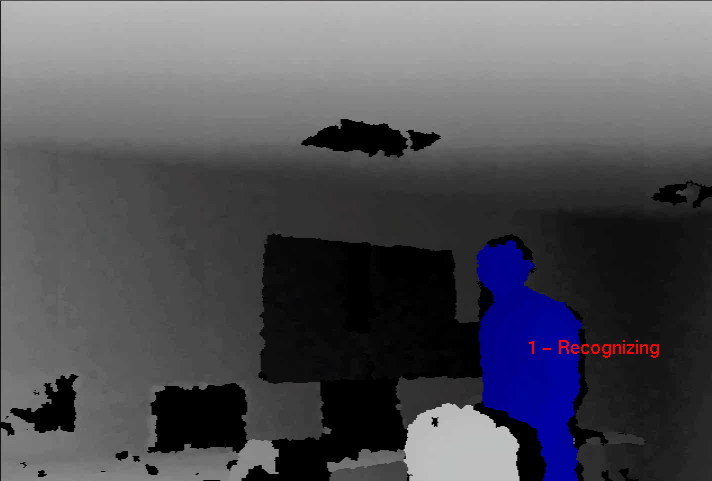
\includegraphics[width=0.25\textwidth]{figuras/5.Testes/deteccao/4.png}}
			\end{center}
			\caption{Momento em que um novo usuário foi detectado pelo Sistema TRUE.}
			\label{fig:testes_deteccao}
		\end{figure}

	Também foram realizados testes para tentar avaliar o impacto da oclusão no rastreamento. A oclusão era um problema esperado pois o Sistema TRUE utiliza somente um sensor \textit{Kinect} como dispositivo de entrada. Em alguns testes um usuário se posicionava no ambiente com intuito de ocultar totalmente outro usuário rastreado. Com isso, caso o usuário continuasse oculto, o sistema o dava como perdido. Porém, o sistema se mostrou robusto em casos que a oclusão era parcial, como mostrado na Figura~\ref{fig:testes_oclusao_sucesso} Em outros testes, foi simulada uma situação mais comum: quando um usuário, em movimento, ocultava ou era oculto, por um momento, por outro usuário. Neste caso, o sistema logo conseguia se recuperar e voltar a rastrear o usuário perdido, como mostrado na Figura~\ref{fig:testes_oclusao}.
		
\begin{figure}[htb]
			\begin{center}
				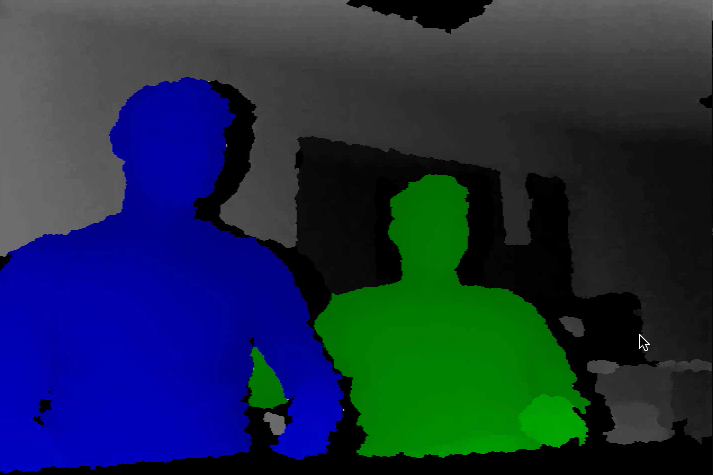
\includegraphics[width=0.75\textwidth]{figuras/5.Testes/oclusao/oclusao_corretamente.png}
			\end{center}
			\caption{Oclusão parcial de dois usuários.}
			\label{fig:testes_oclusao_sucesso}
		\end{figure}
	
		\begin{figure}[htb]
		\begin{center}
				\subfloat[] {
					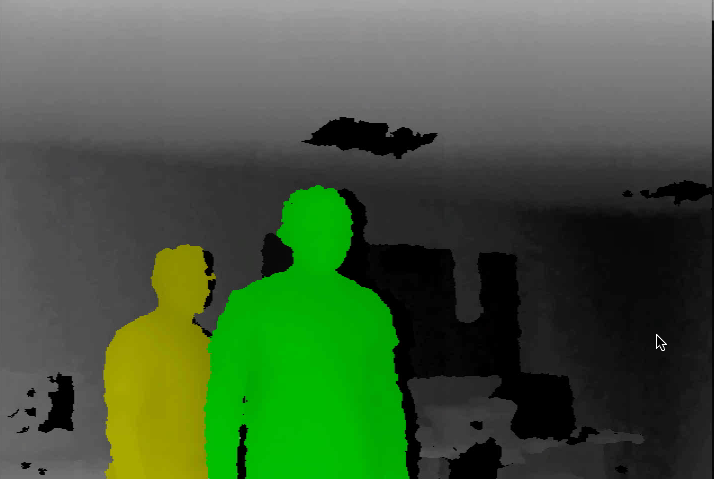
\includegraphics[width=0.19\textwidth]{figuras/5.Testes/oclusao/1.png}}
				\subfloat[] {
					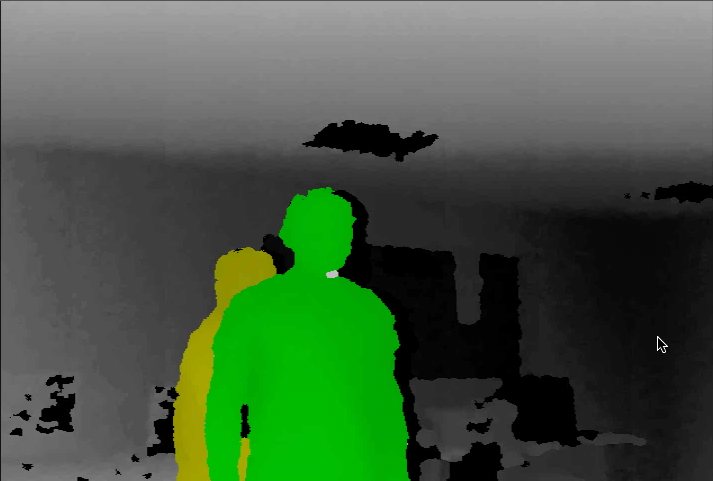
\includegraphics[width=0.19\textwidth]{figuras/5.Testes/oclusao/2.png}}
				\subfloat[] {
					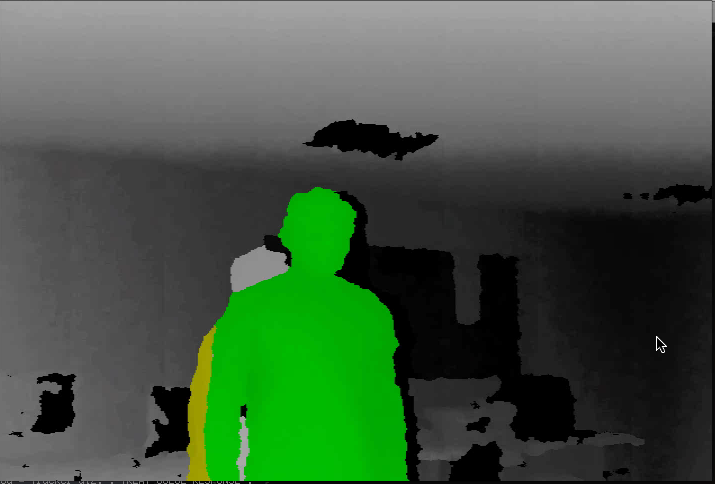
\includegraphics[width=0.19\textwidth]{figuras/5.Testes/oclusao/3.png}}
				\subfloat[] {
					\label{fig:testes_oclusao_ocluso}
					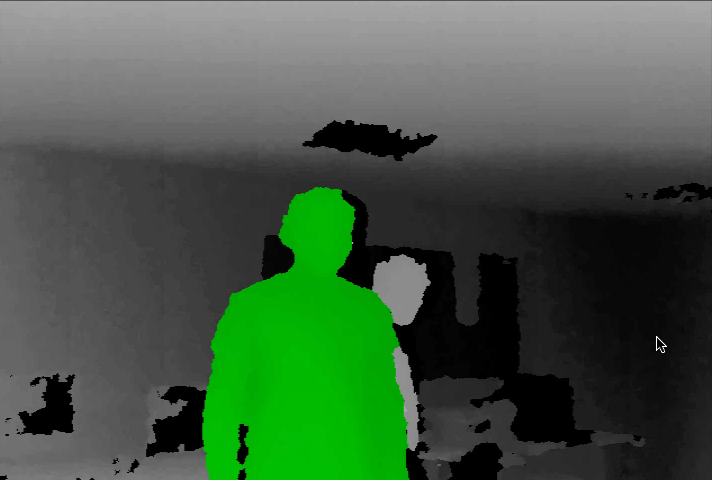
\includegraphics[width=0.19\textwidth]{figuras/5.Testes/oclusao/4.png}}
				\subfloat[] {
					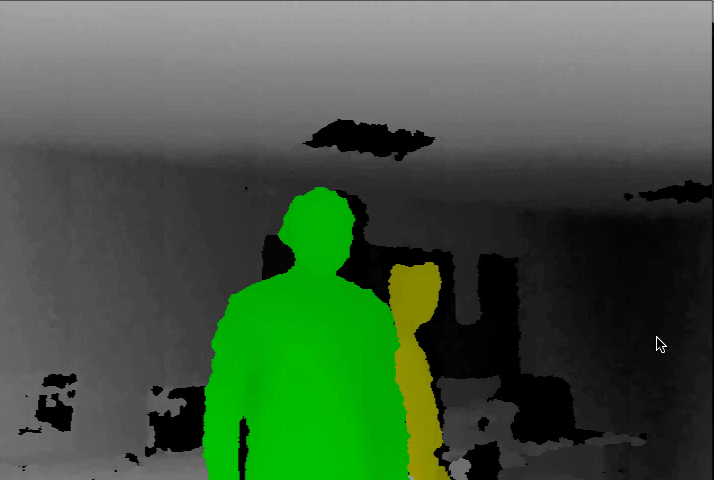
\includegraphics[width=0.19\textwidth]{figuras/5.Testes/oclusao/5.png}}
			\end{center}
			\caption{Oclusão de usuários.}
			\label{fig:testes_oclusao}
		\end{figure}

	Outra caracterísitca importante que foi testada é a abrangência do campo de
	visão do Sistema TRUE. Como já mensionado o sistema utiliza o sensor
	\textit{Kinect} que possui um campo de visão horizontal de 57º. Então, a uma
	distância de, aproximadamente, 4 metros do sensor, o número máximo de usuários
	que cabem no campo de visão sem que haja oclusão são 5 pessoas, como mostrado
	na Figura~\ref{fig:max-pessoas}.

	\begin{figure}[htb]
			\begin{center}
				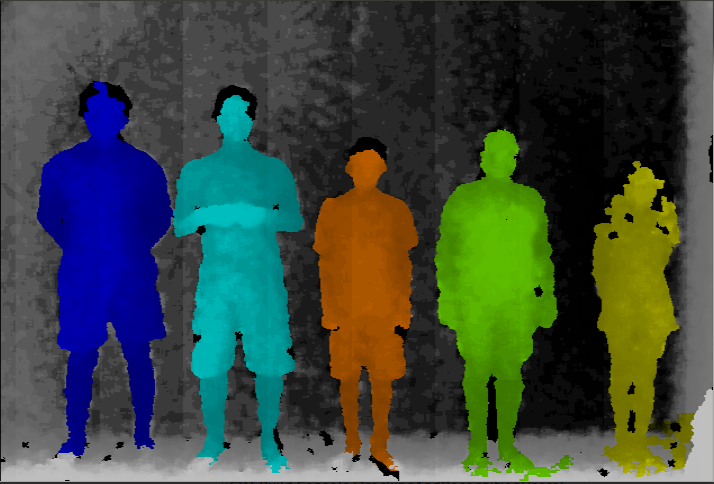
\includegraphics[width=0.4\textwidth]{figuras/5.Testes/oclusao/max-pessoas.png}
			\end{center}
			\caption{Usuários posicionados lado a lado do sensor \textit{Kinect} a uma distância de 4 metros.}
			\label{fig:max-pessoas}
		\end{figure}
		
	Durante os testes realizados com rastreamento foi observado alguns problemas que ocorriam quando o usuário rastreado interagia com objetos ou com outros usuários. Na grande parte das vezes que o usuário interagia com objetos, o Sistema TRUE considerava o objeto como sendo parte do usuário como exemplificado na Figura~\ref{fig:testes_relacionamento_com_objetos}, o que não prejudicou a eficiência do sistema. Já os problemas com interação entre usuários eram bem mais raros, porém o impacto era maior. Esses problemas consistem em algumas ``interferências'' que podiam acontecer quando havia contato entre dois ou mais usuários. A Figura~\ref{fig:testes_relacionamento_com_usuarios} exemplifica melhor essas ``interferências''.
	
		\begin{figure}[htb]
			\begin{center}
				\subfloat[] {
					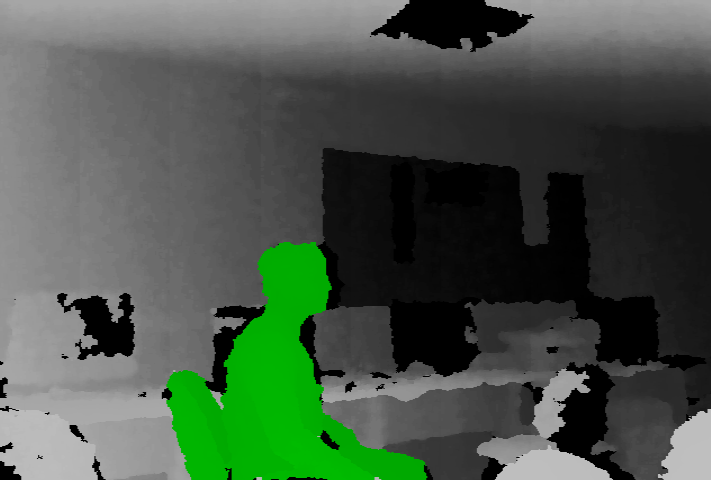
\includegraphics[width=0.37\textwidth]{figuras/5.Testes/relacionamento_com_objetos/1.png}}
				\subfloat[] {
					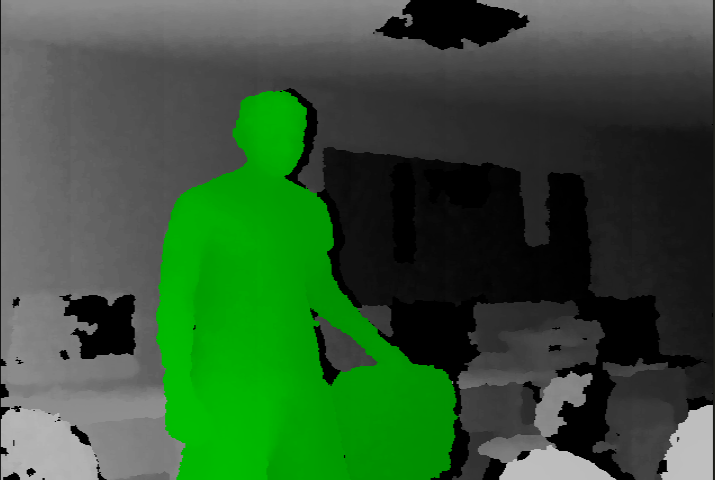
\includegraphics[width=0.37\textwidth]{figuras/5.Testes/relacionamento_com_objetos/2.png}}
			\end{center}
			\caption{Usuários sendo rastreado conjuntamente com os objetos que
			interagem.}
			\label{fig:testes_relacionamento_com_objetos}
		\end{figure}
		
		\begin{figure}[htb]
			\begin{center}
				\subfloat[] {
					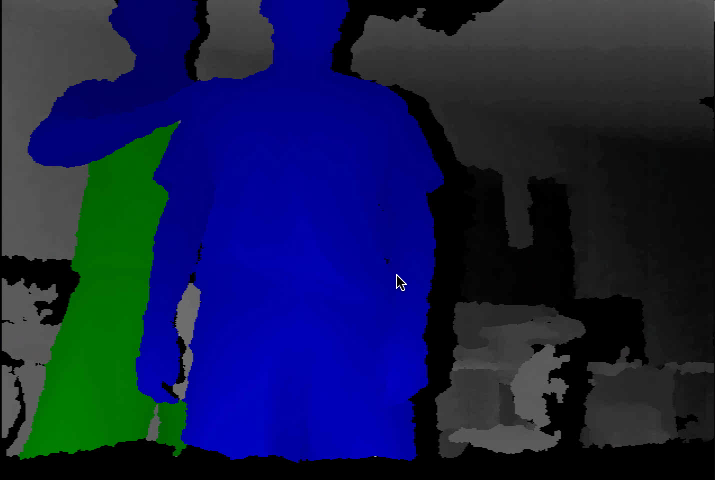
\includegraphics[width=0.32\textwidth]{figuras/5.Testes/relacionamento_com_pessoas/1.png}}
				\subfloat[] {
					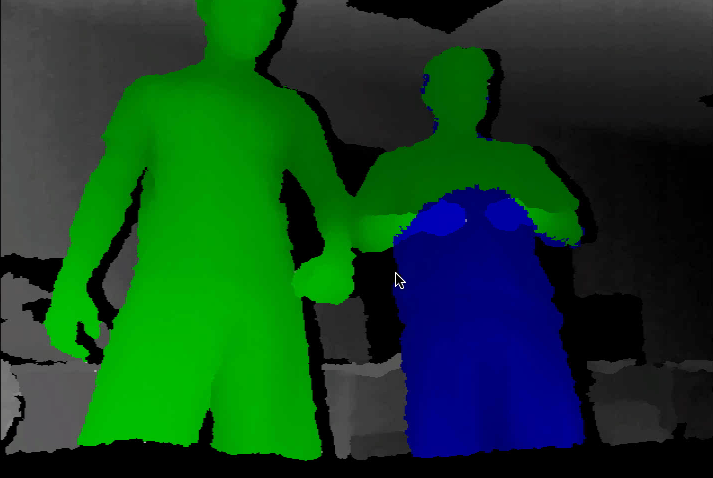
\includegraphics[width=0.32\textwidth]{figuras/5.Testes/relacionamento_com_pessoas/2.png}}
				\subfloat[] {
					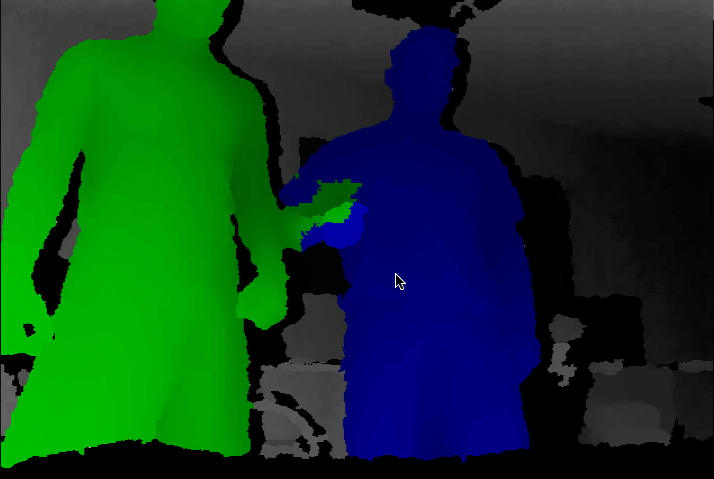
\includegraphics[width=0.32\textwidth]{figuras/5.Testes/relacionamento_com_pessoas/3.png}}
			\end{center}
			\caption{Usuários sofrendo interferência dos que estão ao seu redor.}
			\label{fig:testes_relacionamento_com_usuarios}
		\end{figure}

	Apesar dos problemas relatados, o rastreamento conseguiu, na maioria dos testes, atender as necessidades rastreando os diversos usuários no ambiente em suas atividades diárias, como mostrado na Figura~\ref{fig:varios-usuarios-ambiente}.

	\begin{figure}[htb]
			\begin{center}
				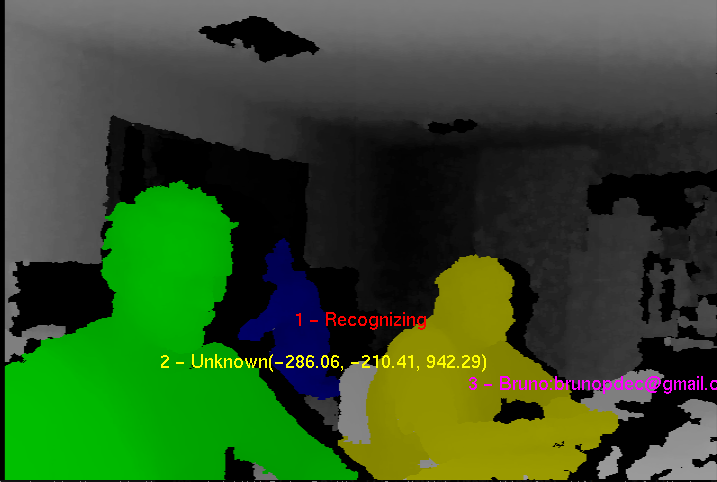
\includegraphics[scale=0.5]{figuras/5.Testes/oclusao/usuarios-rastreados.png}
			\end{center}
			\caption{Usuários rastreados pelo Sistema TRUE.}
			\label{fig:varios-usuarios-ambiente}
		\end{figure}
		
	